\documentclass{sig-alternate-05-2015}
\usepackage{paralist}
\usepackage{tikz}
\usepackage{float}
\usepackage{graphicx}
\usepackage{subcaption}
\usepackage{multirow}

%%%%%%%%%%%%%%%%%%%%%%%%%%%%%%%%%%%%%%%%%%%%%%%%%%%%%%%%%%%%%%%%%%%%%%%%%%%%%%%%
\begin{document} %%%%%%%%%%%%%%%%%%%%%%%%%%%%%%%%%%%%%%%%%%%%%%%%%%%%%%%%%%%%%%%
\setcopyright{acmcopyright}
\conferenceinfo{MMSys '16}{May 10--13, 2016, Klagenfurt am W\"{o}rthersee, Austria}
\doi{}
\isbn{}
%\acmPrice{}

\title{Vertical Search Constraints in Multiview Motion Compensation}
\numberofauthors{2}
\author{
\alignauthor
Ben Hamlin\\
       \affaddr{Portland State University}\\
       \affaddr{Department of Computer Science}\\
       \affaddr{P.O. Box 751}\\
       \affaddr{Portland, OR 97207}\\
       \email{hamlinb@cs.pdx.edu}
\alignauthor
Wuchi Feng\\
       \affaddr{Portland State University}\\
       \affaddr{Department of Computer Science}\\
       \affaddr{P.O. Box 751}\\
       \affaddr{Portland, OR 97207}\\
       \email{wuchi@cs.pdx.edu}
}

\maketitle

\begin{abstract}
Multiview video coding is an important technology for enabling streaming
stereoscopic video, among other applications. However, encoding multiple
views into one stream compounds the size and computation overhead of
traditional video coding. Because of this, there is a need to come up with new
ways to improve the space-time trade-off inherent in multiview video coding. In
this paper, we present a systematic analysis of the trade-offs between
computation time and bit-rate with respect to inter-view motion-compensation.
In addition, we propose a method of constraining inter-view motion-vector search
that leverages the relationship between views to speed up search times by a factor
of two for views with one reference and a factor of four for views with two
references over using a modern fast search algorithm alone, with at most a small
increase in bit-rate.
\end{abstract}

\begin{CCSXML}
<ccs2012>
<concept>
<concept_id>10002951.10003227.10003251</concept_id>
<concept_desc>Information systems~Multimedia information systems</concept_desc>
<concept_significance>500</concept_significance>
</concept>
</ccs2012>
\end{CCSXML}
\ccsdesc[500]{Information systems~Multimedia information systems}
\printccsdesc

\keywords{Video coding; Motion compensation; Multiview}

\section{Introduction} %%%%%%%%%%%%%%%%%%%%%%%%%%%%%%%%%%%%%%%%%%%%%%%%%%%%%%%%%
\label{sec:introduction} %%%%%%%%%%%%%%%%%%%%%%%%%%%%%%%%%%%%%%%%%%%%%%%%%%%%%%%
Multiview video coding (MVC) is a field that has emerged in the last two decades
to enable technologies such as stereoscopic video and free-viewpoint video. In
stereoscopic video, views from different, horizontally separated cameras are
presented to each eye to simulate a 3-dimensional scene. It is frequently useful
to have more than 2 views available to compensate for the viewer's distance from
the screen. Free-viewpoint video uses the views from multiple horizontally
separated cameras to allow the user to choose his vantage point on a scene. In
either case, it is necessary to encode at least two video streams together.

Multiview video presents bandwidth and storage challenges, since it is obviously
more expensive to transport or store multiple viewpoints than it is to transport
or store just one. Fortunately, since all the cameras are focused on the same
scene there is some inter-view redundancy, which can be taken advantage of such
that the combined views can be encoded more efficiently together than they could
be individually.

The mechanism commonly used -- most pertinently, in ITU/ISO H.264/MPEG4 AVC
and Annex H, its multiview extension -- is block-based motion compensation. This
allows some pictures to be stored with reference to one or two other pictures.
Each block of the dependent view can optionally be stored as a spatial offset,
at up to quarter-pixel resolution, to a similar block in the reference view and
a frequency-domain difference between the dependent and reference blocks.

With this technique, the encoder can reduce inter-view redundancy and save
space, but at the cost of spending time searching the reference pictures for
similar blocks. In general, increasing the search space decreases the resulting
bit-rate, but takes more time. It's reasonable then, to ask what the best
trade-off is between time and efficiency. A variety of algorithms exist to
decrease the subset of blocks to search (a survey of several existing
algorithms, as well as two novel ones, is presented in \cite{khattak:fast}),
many of which have achieved impressive results. In general, these take a
divide-and-conquer approach, searching in a fixed set of locations around some
center point at smaller and smaller granularities.

Another approach -- the one we explore in this paper -- would be to use
knowledge about the constrained set of ways in which the views can differ from
each other to narrow down the possibilities before searching. Specifically,
in the common case, the cameras taking the different views are located in the
same horizontal plane. This means that objects that are non-occluded in both
views will have different x-coordinates, but will never have different
y-coordinates. We propose constraining the inter-view motion-vector search to
consider only horizontal motion-vector offsets, not vertical ones. Note that
this is complementary to existing motion-vector search algorithms. In our
experiments, this produced approximately a two-times speedup for views with
one reference and about a four-times speedup for views with two references
over using a fast search algorithm alone, while incurring between $0\%$ and
$7\%$ increase in bit-rate depending on the content of the video.

In addition, the structure of the view dependencies can have a profound effect
on the efficiency with which the dependent views are coded. For example, we
found in our experiments that a view that depended on a reference two views away
took up nearly twice as much space on average as one whose reference was only
one view away. Perhaps more surprisingly still, when a view's reference was five
views away it actually had a higher bit-rate than the average independent view,
which means that encoding a view in this way is never worthwhile. An ideal view
dependency structure would never make a view depend on a reference more than one
view away. If the number of views is large, however, this could require that
views be made hierarchical. But in stereoscopic video, for example, it may be
desirable to separate out just two views to transport, and having hierarchical
view dependencies makes this expensive.

The contributions of this work are twofold: \begin{compactitem}
\item We present experimental data on the time taken and bit-rates achieved by a
variety of view-dependency structures, arriving at a suggestion for an optimal
8-view dependency structure and an intuition about in which cases unidirectional
and bidirectional inter-view dependencies are useful.
\item We introduce the idea of vertical search constraints for inter-view motion
vectors and provide experimental data that demonstrates the kinds of speedups
and bit-rates it can achieve. \end{compactitem} To our knowledge, this is the
first paper to explore vertically constraining inter-view motion compensation.
It is also the first to provide a systematic analysis of the time and bit-rates
required by various view structures under H.264 Annex H, and to  characterize
them according to their distance from their reference views, although
\cite{merkle:efficient} gives an excellent characterization of the relative
efficiencies of inter and inter-view motion compensation. In performing our
experiments, we additionally identified a bug in the JMVC, the H.264 MVC
reference codec \cite{schwarz:jmvc}, which we have reported to the project's
maintainers.

The remainder of this paper is organized as follows: Section
\ref{sec:background} provides some background information on multiview coding.
We describe our results and the methods we used to obtain them in sections
\ref{sec:results} and \ref{sec:method}, respectively. Finally, in section
\ref{sec:conclusion} we sum up.

\section{Background} %%%%%%%%%%%%%%%%%%%%%%%%%%%%%%%%%%%%%%%%%%%%%%%%%%%%%%%%%%%
\label{sec:background} %%%%%%%%%%%%%%%%%%%%%%%%%%%%%%%%%%%%%%%%%%%%%%%%%%%%%%%%%

In this section, we describe two of the key features of multiview coding that
we refer to in the remainder of the paper. In \ref{subsec:motion} we
describe motion compensation and how it is used in the base H.264 standard and
in MVC. In \ref{subsec:depends}, we discuss frame and view dependency
structures for motion compensation and describe some of the things that must  be
taken into account when deciding what structures to use.

\subsection{Motion Compensation}
\label{subsec:motion}

Block-based motion compensation is a technique for reducing redundancies in two
pictures by encoding some or all of one with reference to the other. H.264 uses
a method similar to JPEG for encoding independent pictures. Pictures are divided
into blocks of varying sizes, each of which is transformed into the frequency
domain and stored as a set of coefficients to horizontally and vertically
oriented sinusoidal functions. These coefficients can then be quantized
to reduce the image's quality in ways that are difficult for the human eye to
perceive. H.264 uses block sizes of $16\times 16$, $16\times 8$, $8\times 16$,
or $8\times 8$ ($w\times h$). Breaking images into blocks in this way lends
itself naturally to block-wise encoding of inter-picture similarities.

Once the dependent picture has been divided into blocks in this way, and the
block sizes have been chosen based on the content of each $16\times 16$
macroblock, the reference picture is searched for similar blocks of the same
size at up to quarter-pixel resolution. The encoder has two other options for
each macroblock, as well. If no suitable motion vector is found, it can choose
to independently encode the macroblock in the same way it would be encoded in an
independent picture. Alternatively, if the macroblock is identical to the
spatially corresponding one in the reference frame, it can be {\it skipped},
meaning the decoder will just take it directly from the reference frame.

If a suitable block is found, it is encoded as the spatial offset (in
quarter-pixels) from the dependent block to the reference block (the {\it motion
vector}). The encoder then takes the frequency-domain coefficient-wise
difference between the two (the {\it residual}) and encodes it along with the
motion vector. Since the two blocks are similar, these coefficient differences
should be small, allowing them to frequently be quantized down to zero and
efficiently compressed using run-length encoding. If two reference pictures are
present, the encoder may choose a block from each picture, in which case both
motion vectors are stored, and the residual is the difference between each
dependent coefficient and the average of each pair of reference coefficients.

Note that the standard does not specify how this search should occur, only how
the result should be encoded. One approach would be to do an exhaustive search
of all possible reference blocks and reference block combinations. In the worst
case, this involves $B \times Q$ comparisons per picture with one reference, and
$2(B \times Q) + B \times Q^2$ comparisons with two (where $Q = 4(W\times H)$ is
the number of quarter pixels in the image and $B$ is the number of blocks, of
varying size).

This search is generally the most time-consuming part of the video coding
process, so encoders usually take a number of measures to narrow down the search
space. The first and most obvious step is to limit the search radius. Thus
encoders usually specify a square around the original block to search (e.g.,
$64\times 64$ pixels. Another approach (called {\it raster search}) is to reduce
the resolution of the search, so that only one block is searched in a fixed-size
neighborhood. A third approach is to search in a fixed pattern (usually a
square, diamond, pentagon, hexagon, etc.) around a center point. The point
chosen becomes the new center, and the search is repeated with a decreased
radius, until at some point, the search finishes with a quarter-pixel full
search of some small area.

These approaches assume that the best reference block is most likely to be
within a small area around the dependent block. This assumption is reasonable
in the case of motion compensation in the base H.264 standard, where reference
pictures are temporally offset by one or a few frames within the same video
stream ({\it inter} coding). Since a smoothly moving object is only likely to
travel a small number of pixels between frames, the new block containing it is
likely to be close to the old one. Of course, motion vectors aren't limited to
encoding actual motion. They can also encode visual similarities between blocks
whose content is unrelated, meaning that the best reference block is sometimes
distant from the dependent block.

Stronger assertions can be made when using motion compensation to encode
temporally corresponding pictures within different views ({\it inter view}
coding). Assuming the views are being used for stereoscopic or free-viewpoint
video, objects shared between views always lie within the same horizontal plane.
In addition pictures from different views are always correlated. They are not
subject, for example, to being separated by scene changes. The only case in
which an object can be in one view but not in another is when it is occluded. It
is this insight that leads us to propose vertically constraining motion-vector
search.

\subsection{View-Dependency Structures}
\label{subsec:depends}
In order to take advantage of spatial redundancy using inter-view motion
compensation, the encoder needs to make a number of choices. It needs to decide
which views will be independent and which won't. Then for each dependent view,
it must determine whether that view should have one reference or two and which
views those references should be. (Note that it's usually the user who actually
makes this choice, not the encoder software.) In general, independent views are
the least time-consuming, but take up the most space, bidirectionally coded views
take up the least space but take the most time, and unidirectionally coded views
are in the middle.

Within a view, pictures are organized into groups (GOPs), which consist of a set
of pictures that can be decoded on their own, without reference to previous
pictures from the same view \cite{vetro:overview}. An example of this is given in
figure \ref{fig:inter}, where the GOP-size is 4.

\begin{figure}[H]
\begin{center}
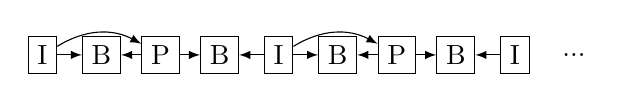
\begin{tikzpicture}[scale=0.75,every path/.style={>=latex},every node/.style={draw,rectangle}]
\node            (a) at (0,0)  { I };
\node            (b) at (1,0)  { B };
\node            (c) at (2,0)  { P };
\node            (d) at (3,0)  { B };
\node            (e) at (4,0)  { I };
\node            (f) at (5,0)  { B };
\node            (g) at (6,0)  { P };
\node            (h) at (7,0)  { B };
\node            (i) at (8,0)  { I };
\node[draw=none]     at (9,0)  { ... };
\draw[->]            (a) edge (b);
\draw[->]            (c) edge (b);
\draw[->, bend left] (a) edge (c);
\draw[->]            (c) edge (d);
\draw[->]            (e) edge (d);
\draw[->]            (e) edge (f);
\draw[->]            (g) edge (f);
\draw[->, bend left] (e) edge (g);
\draw[->]            (g) edge (h);
\draw[->]            (i) edge (h);
\end{tikzpicture}
\end{center}
\caption{
A typical inter-coding structure with GOP size 4. \\
Arrows point from the reference to the dependent picture.
}
\label{fig:inter}
\end{figure}

In dependent views, it is common for every picture to have at least one
inter-view reference and every picture but the first to additionally be
inter-coded (\cite{vetro:overview}, \cite{khattak:fast}, e.g.). An example is
given in figure \ref{fig:inter-view}. This allows the encoder to take
advantage of both spatial and temporal redundancies in a dependent view.

\begin{figure}[H]
\begin{center}
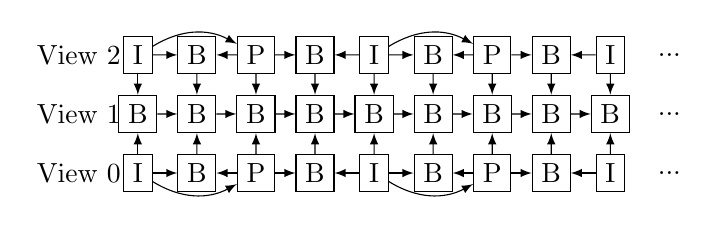
\begin{tikzpicture}[scale=0.75,every path/.style={>=latex},every node/.style={draw,rectangle}]
\node[draw=none]      at (-1,0) { View 0 };
\node            (a0) at (0,0)  { I };
\node            (b0) at (1,0)  { B };
\node            (c0) at (2,0)  { P };
\node            (d0) at (3,0)  { B };
\node            (e0) at (4,0)  { I };
\node            (f0) at (5,0)  { B };
\node            (g0) at (6,0)  { P };
\node            (h0) at (7,0)  { B };
\node            (i0) at (8,0)  { I };
\node[draw=none]      at (9,0)  { ... };
\node[draw=none]      at (-1,1) { View 1 };
\node            (a1) at (0,1)  { B };
\node            (b1) at (1,1)  { B };
\node            (c1) at (2,1)  { B };
\node            (d1) at (3,1)  { B };
\node            (e1) at (4,1)  { B };
\node            (f1) at (5,1)  { B };
\node            (g1) at (6,1)  { B };
\node            (h1) at (7,1)  { B };
\node            (i1) at (8,1)  { B };
\node[draw=none]      at (9,1)  { ... };
\node[draw=none]      at (-1,2) { View 2 };
\node            (a2) at (0,2)  { I };
\node            (b2) at (1,2)  { B };
\node            (c2) at (2,2)  { P };
\node            (d2) at (3,2)  { B };
\node            (e2) at (4,2)  { I };
\node            (f2) at (5,2)  { B };
\node            (g2) at (6,2)  { P };
\node            (h2) at (7,2)  { B };
\node            (i2) at (8,2)  { I };
\node[draw=none]      at (9,2)  { ... };
\draw[->]             (a0) edge (b0);
\draw[->]             (c0) edge (b0);
\draw[->, bend right] (a0) edge (c0);
\draw[->]             (c0) edge (d0);
\draw[->]             (e0) edge (d0);
\draw[->]             (e0) edge (f0);
\draw[->]             (g0) edge (f0);
\draw[->, bend right] (e0) edge (g0);
\draw[->]             (g0) edge (h0);
\draw[->]             (i0) edge (h0);
\draw[->]             (a0) edge (a1);
\draw[->]             (b0) edge (b1);
\draw[->]             (c0) edge (c1);
\draw[->]             (d0) edge (d1);
\draw[->]             (e0) edge (e1);
\draw[->]             (f0) edge (f1);
\draw[->]             (g0) edge (g1);
\draw[->]             (h0) edge (h1);
\draw[->]             (i0) edge (i1);
\draw[->]             (a1) edge (b1);
\draw[->]             (b1) edge (c1);
\draw[->]             (c1) edge (d1);
\draw[->]             (d1) edge (e1);
\draw[->]             (e1) edge (f1);
\draw[->]             (f1) edge (g1);
\draw[->]             (g1) edge (h1);
\draw[->]             (h1) edge (i1);
\draw[->]             (a2) edge (a1);
\draw[->]             (b2) edge (b1);
\draw[->]             (c2) edge (c1);
\draw[->]             (d2) edge (d1);
\draw[->]             (e2) edge (e1);
\draw[->]             (f2) edge (f1);
\draw[->]             (g2) edge (g1);
\draw[->]             (h2) edge (h1);
\draw[->]             (i2) edge (i1);
\draw[->]             (a2) edge (b2);
\draw[->]             (c2) edge (b2);
\draw[->, bend left]  (a2) edge (c2);
\draw[->]             (c2) edge (d2);
\draw[->]             (e2) edge (d2);
\draw[->]             (e2) edge (f2);
\draw[->]             (g2) edge (f2);
\draw[->, bend left]  (e2) edge (g2);
\draw[->]             (g2) edge (h2);
\draw[->]             (i2) edge (h2);
\end{tikzpicture}
\end{center}
\caption{
A typical view-internal coding structure
with both dependent and reference pictures. \\
Pictures are both inter-coded and inter-view coded.
}
\label{fig:inter-view}
\end{figure}

In our tests, we chose to do away with the inter-coding in dependent views. We
did this for two reasons. First, the JMVC reference codec does not support
pictures that are both inter and inter-view coded in any configurable way.
Instead, it uses the same GOP structure for both dependent and reference views,
with inter-view coded pictures in place of I-frames. More importantly, however,
doing away with inter-coding in the dependent views allows us to isolate the
coding efficiency achieved by inter-view coding alone, without having to worry
about the noise introduced by variable temporal redundancy. From here on, we
assume that all dependent and independent views have internal structures as
shown in figure \ref{fig:just-inter-view}.

\begin{figure}[H]
\begin{center}
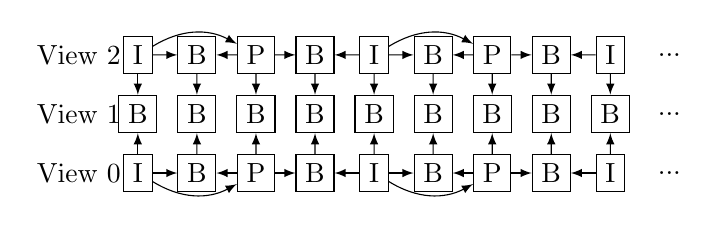
\begin{tikzpicture}[scale=0.75,every path/.style={>=latex},every node/.style={draw,rectangle}]
\node[draw=none]      at (-1,0) { View 0 };
\node            (a0) at (0,0)  { I };
\node            (b0) at (1,0)  { B };
\node            (c0) at (2,0)  { P };
\node            (d0) at (3,0)  { B };
\node            (e0) at (4,0)  { I };
\node            (f0) at (5,0)  { B };
\node            (g0) at (6,0)  { P };
\node            (h0) at (7,0)  { B };
\node            (i0) at (8,0)  { I };
\node[draw=none]      at (9,0)  { ... };
\node[draw=none]      at (-1,1) { View 1 };
\node            (a1) at (0,1)  { B };
\node            (b1) at (1,1)  { B };
\node            (c1) at (2,1)  { B };
\node            (d1) at (3,1)  { B };
\node            (e1) at (4,1)  { B };
\node            (f1) at (5,1)  { B };
\node            (g1) at (6,1)  { B };
\node            (h1) at (7,1)  { B };
\node            (i1) at (8,1)  { B };
\node[draw=none]      at (9,1)  { ... };
\node[draw=none]      at (-1,2) { View 2 };
\node            (a2) at (0,2)  { I };
\node            (b2) at (1,2)  { B };
\node            (c2) at (2,2)  { P };
\node            (d2) at (3,2)  { B };
\node            (e2) at (4,2)  { I };
\node            (f2) at (5,2)  { B };
\node            (g2) at (6,2)  { P };
\node            (h2) at (7,2)  { B };
\node            (i2) at (8,2)  { I };
\node[draw=none]      at (9,2)  { ... };
\draw[->]             (a0) edge (b0);
\draw[->]             (c0) edge (b0);
\draw[->, bend right] (a0) edge (c0);
\draw[->]             (c0) edge (d0);
\draw[->]             (e0) edge (d0);
\draw[->]             (e0) edge (f0);
\draw[->]             (g0) edge (f0);
\draw[->, bend right] (e0) edge (g0);
\draw[->]             (g0) edge (h0);
\draw[->]             (i0) edge (h0);
\draw[->]             (a0) edge (a1);
\draw[->]             (b0) edge (b1);
\draw[->]             (c0) edge (c1);
\draw[->]             (d0) edge (d1);
\draw[->]             (e0) edge (e1);
\draw[->]             (f0) edge (f1);
\draw[->]             (g0) edge (g1);
\draw[->]             (h0) edge (h1);
\draw[->]             (i0) edge (i1);
\draw[->]             (a2) edge (a1);
\draw[->]             (b2) edge (b1);
\draw[->]             (c2) edge (c1);
\draw[->]             (d2) edge (d1);
\draw[->]             (e2) edge (e1);
\draw[->]             (f2) edge (f1);
\draw[->]             (g2) edge (g1);
\draw[->]             (h2) edge (h1);
\draw[->]             (i2) edge (i1);
\draw[->]             (a2) edge (b2);
\draw[->]             (c2) edge (b2);
\draw[->, bend left]  (a2) edge (c2);
\draw[->]             (c2) edge (d2);
\draw[->]             (e2) edge (d2);
\draw[->]             (e2) edge (f2);
\draw[->]             (g2) edge (f2);
\draw[->, bend left]  (e2) edge (g2);
\draw[->]             (g2) edge (h2);
\draw[->]             (i2) edge (h2);
\end{tikzpicture}
\end{center}
\caption{
The view-internal structure we use in our tests. \\
Pictures in the dependent view use inter-view coding only.
}
\label{fig:just-inter-view}
\end{figure}

With the view-internal coding structure established, we can now turn our
attention to the inter-view coding structure. There is little consensus in
the literature about what inter-view structure is best. In section
\ref{sec:results}, we propose some optimal frame structures as adduced from the
results of our experiments.

\section{Experimental Method} %%%%%%%%%%%%%%%%%%%%%%%%%%%%%%%%%%%%%%%%%%%%%%%%%%
\label{sec:method} %%%%%%%%%%%%%%%%%%%%%%%%%%%%%%%%%%%%%%%%%%%%%%%%%%%%%%%%%%%%%
In this section, we describe the methods we used to obtain our results.
Subsections \ref{subsec:jmvc} and \ref{subsec:modifications} talk about the JMVC
reference codec and the modifications we made to it in order to obtain the data
we needed. In the process of performing those modifications, we identified a bug
in the codec, which we describe in \ref{subsec:bug}. Finally, in
\ref{subsec:data-set} and \ref{subsec:environment}, we talk about the data sets
we used and the hardware and software platform we ran our tests on.

\subsection{Codec: JMVC}
\label{subsec:jmvc}
JMVC is the H.264 MVC reference codec \cite{schwarz:jmvc}. It is adapted from
JM \cite{suehring:jm}, the MPEG4/H.264 AVC reference codec. It contains a
complete implementation of the H.264 multiview extensions.

JMVC provides two methods of motion vector search: {\it block search}, which
tests every block in a region around the block being predicted for, and {\it
TZ-search}, which uses a combination of scaled-down raster search and diamond
refinement \cite{purnachand:improvements}. We ran tests using both algorithms,
but we will focus on our results using TZ-search, since this most closely
matches the way the codec would be used in practice.

The codec also has several options when it comes to measuring the similarity
between blocks for motion compensation: sum of absolute differences (SAD); sum
of squared errors (SSE); or Hadamard. We used SAD for our tests, since it is
the simplest to reason about.

\subsection{Our Modifications}
\label{subsec:modifications}
In order to gather data about the coding process, we made the following changes
to the JMVC software:

\begin{enumerate}
\item We instrumented the process of writing motion vectors to the byte-stream
by first writing the same information in human-readable format to a text file.
This allowed us to examine the motion vectors to codec produced and compare them
the motion vectors we expected.

\item We inserted a timer around the process of encoding each picture, which
allowed us to determine exactly what portion of its time JMVC was spending on
each picture type.

\item We added a parameter to the configuration file that allowed us to
vertically constrain the motion-vector search space by a configurable amount.
\end{enumerate}

\subsection{A Bug in JMVC}
\label{subsec:bug}
In the process of making and testing these changes to JMVC, we discovered what
appears to be a bug in how JMVC searches the reference picture for similar
blocks. JMVC allows the motion-vector search space to be limited to a square of
configurable size around the dependent block. In some cases, however, this
square goes off the edge of the picture and must be further restricted to end
at the picture's edges.

In the case where the square went off the top or left edge, JMVC did not
properly constrain this square, resulting in the motion-vector search going out
of the bounds of the array the representing the reference picture. The
resulting garbage would occasionally yield a block that the encoder found
similar enough, resulting in motion vectors that referred to blocks off the
edge of the picture. We have reported this bug to the software's maintainers.

\begin{figure}[H]
\centering
\begin{subfigure}{.5\textwidth}
\centering
\fbox{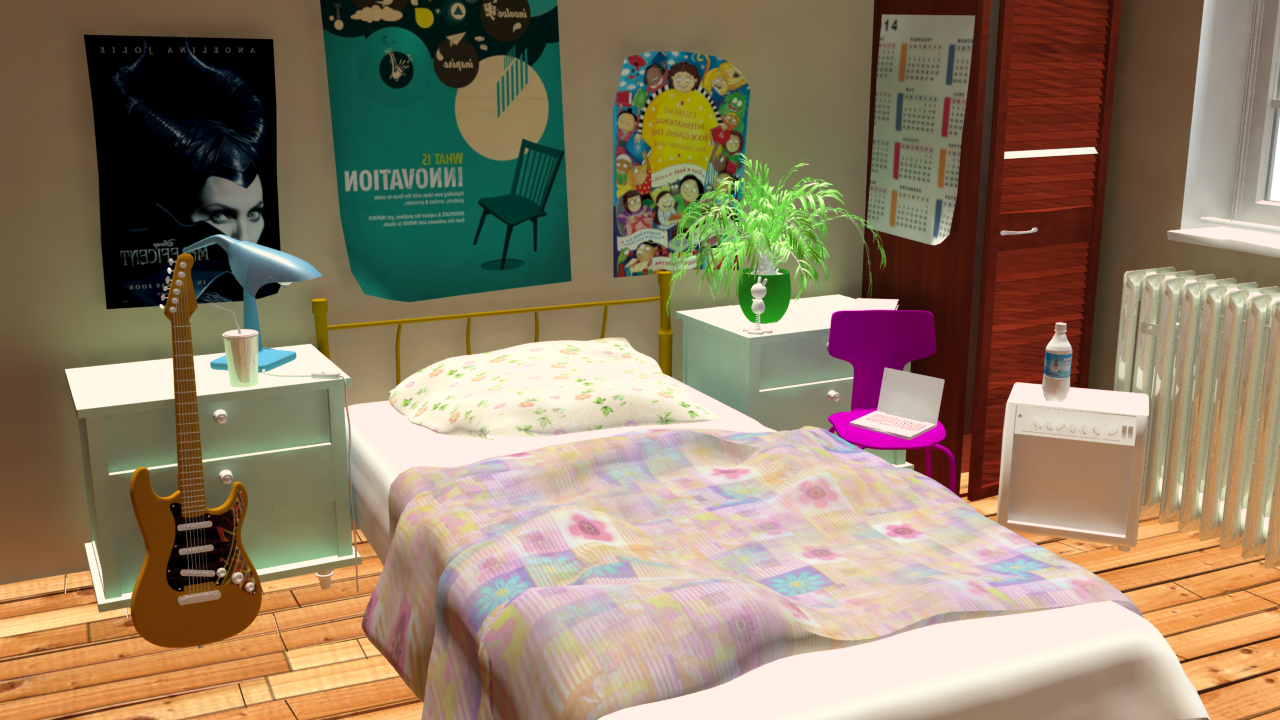
\includegraphics[width=3in]{figures/bedroom1_view0_frame100.png}}
\caption{View 0, frame 100 of bedroom data set.}
\end{subfigure} \\
\begin{subfigure}{.5\textwidth}
\centering
\fbox{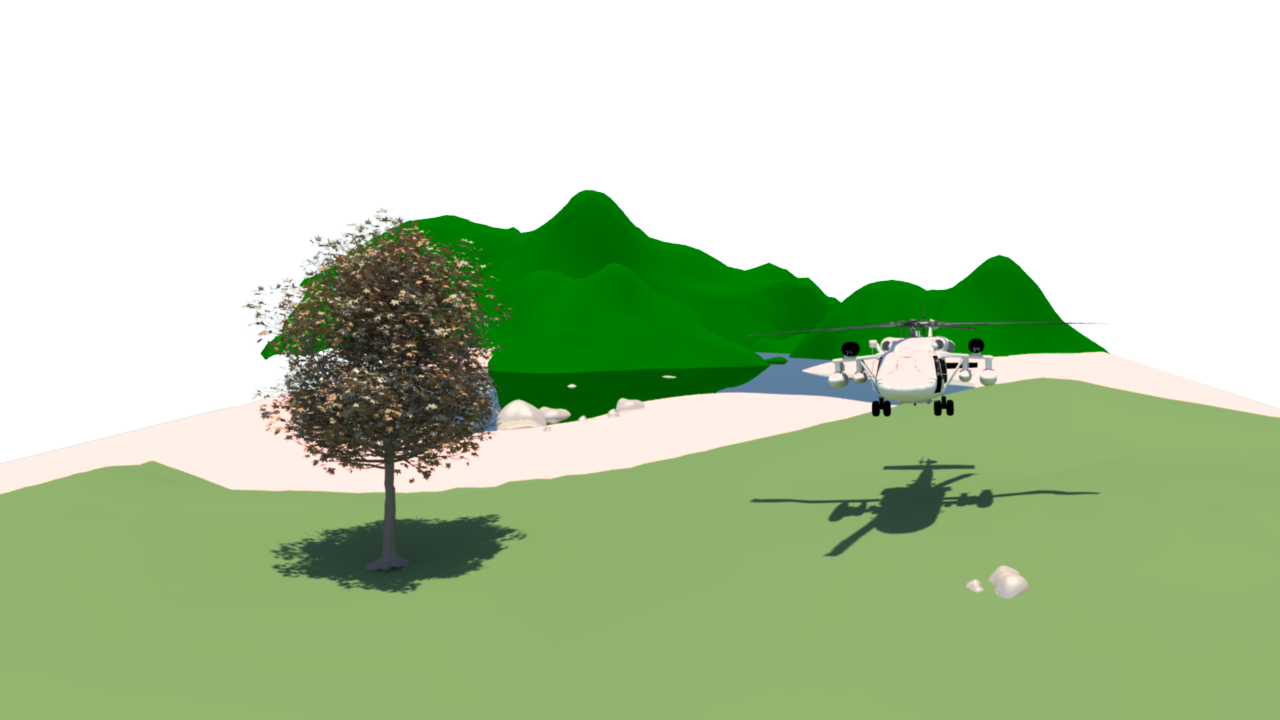
\includegraphics[width=3in]{figures/helicopter_view0_frame100.png}}
\caption{View 0, frame 100 of helicopter data set.}
\end{subfigure}
\caption{A frame from each of the two data sets we used in our tests.}
\label{fig:data-set}
\end{figure}

\subsection{Data Set}
\label{subsec:data-set}
We ran our tests on 3D-rendered data-sets constructed specifically for testing
multi-view coding. We ran tests on two data sets: The first is a scene of a
bedroom, in which the cameras pan horizontally across the room. The second
depicts a helicopter landing. A frame from each data set is shown in figure
\ref{fig:data-set}.

Each view contains 300 frames. Each frame is $1280\times 720$ pixels, and the
views are separated by about 15 pixels. They are meant to simulate separate
viewpoints, so objects in one view may be occluded in another. Our tests in
\ref{subsec:optimal} were run using the first 100 frames from each data-set.
The rest of our tests used all 300 frames.

Using constructed video streams, rather than the output of actual multiview
cameras allows us to avoid artifacts that might occur in real footage. For
example, the cameras might be slightly tilted or out of horizontal alignment,
or one of the cameras might have a flawed lens, decreasing the similarity
between views. Although these are considerations that come up in practice,
our interest is in gathering data about the common case, where the views
have the expected correlation.

We performed our timing tests for vertically constrained versus unconstrained
search using two view configurations. The first was the simplest configuration
possible: two views in which the first is the reference view, and the second
is dependent on the first. In addition to this, we ran tests on two eight-view
configurations. The structures of these and what motivated us to choose them
are described in \ref{subsec:optimal}.

\subsection{Testing Environment}
\label{subsec:environment}
All of our tests were performed on Red Hat Enterprise Linux version 4.1.2-54
using the SMP build of kernel version 2.6.18-371.6.1.el5. We encoded the YUV
files we used as input to JMVC using ffmpeg version 0.6.5. We compiled JMVC
with {\tt -O2} using gcc version 4.1.2. Our times were collected using GNU Time
version 1.7 for the per-view encoding times and {\tt clock\_gettime()} using
Linux's {\tt CLOCK\_MONOTONIC} for per-picture timing. Our hardware platforms
were servers with two hyper-threaded 4-core 2.4Ghz Intel Xeon processors. These
had cache sizes of 12288KB.

\section{Results} %%%%%%%%%%%%%%%%%%%%%%%%%%%%%%%%%%%%%%%%%%%%%%%%%%%%%%%%%%%%%%
\label{sec:results} %%%%%%%%%%%%%%%%%%%%%%%%%%%%%%%%%%%%%%%%%%%%%%%%%%%%%%%%%%%%
In this section, we present the results of our experiments and use them to make
judgements about how best to organize view dependencies, when to use
unidirectionally and bidirectionally coded views, and whether applying vertical
constraints to the motion-vector search of dependent views is worthwhile. The
former two points are discussed in subsection \ref{subsec:optimal}, while the
latter point is motivated and discussed in subsections
\ref{subsec:unconstrained} and \ref{subsec:constrained}, respectively.

\subsection{Finding the Optimal View Structure}
\label{subsec:optimal}
We knew from the outset that we wanted to test our constrained motion-vector
search under two scenarios. The first was the simple case of two adjacent views,
one depending on the other. This would let us determine the fundamental costs
and benefits of vertical constraints in a simple, idealized scenario. The view
structure that this scenario requires is obvious, and allows for no
optimization.

It is frequently desirable to encode more than two views, however, in order to
implement free-viewpoint video, for example, or in order to adjust the distance
of two stereoscopic views according to the user's proximity to the screen. To
model this scenario, we also wanted to perform tests using eight views. In this
case, however, it is far from obvious what the best choice of view structure
might be.

Since JMVC encodes at a variable bit-rate, there are two variables to optimize
for: bit-rate and time. In terms of time, the optimal configuration is to not
use motion compensation at all and make every view independent. This completely
fails to take advantage of spatial and temporal redundancies, however, and
requires a prohibitively high bit-rate. In order to reason about what view
structures are most computationally efficient, it is necessary to know the
time taken by each kind of view. Figure \ref{fig:view-type-times} shows
the average time taken to encode each view type.

\begin{figure}
\centering
\begin{tabular}{|l|r|}
\hline
view type               & mean encoding time (seconds) \\
\hline
independent             & 465.13                       \\
dependent, 1 reference  & 348.99                       \\
dependent, 2 references & 1339.34                      \\
\hline
\end{tabular}
\caption{Time to encode 100 frames of each view type averaged over 10 trials
with each data-set.}
\label{fig:view-type-times}
\end{figure}

Independent views are a mixture of I-, B-, and P-frames. Since they use the
internal structure described in \ref{subsec:depends}, about half of these
are B-frames. This makes independent views slightly more expensive than
single-reference dependent frames. It's important to note that this would not be
the case if we were using JMVC's default view-internal frame structure, which
structures dependent views the same as independent ones, except with I-frames
replaced by inter-view coded frames (see \ref{subsec:depends}). In that case,
independent frames would be the fastest to encode.

The most important thing to note in figure \ref{fig:view-type-times}, however,
is the relationship between the time it takes to encode dependent views with one
reference as opposed to dependent views with two. Dependent views with two
references take nearly four times as long. This means that from the standpoint
of computation time, bidirectional dependent views should be avoided whenever
possible. In \ref{subsec:constrained} we discuss how constraining the search
space can reduce this gap and make bidirectional dependent views more feasible.

Finding the optimal configuration in terms of bit-rate requires that we know how
many bits, on average, each view type takes for each possible distance from its
reference view or views. We used our modified JMVC to acquire this data. The
bit-rates for single-reference pictures are presented in figure
\ref{fig:uniframes}, and the bit-rates for two-reference pictures are given in
figure \ref{fig:biframes}.

\begin{figure}
\centering
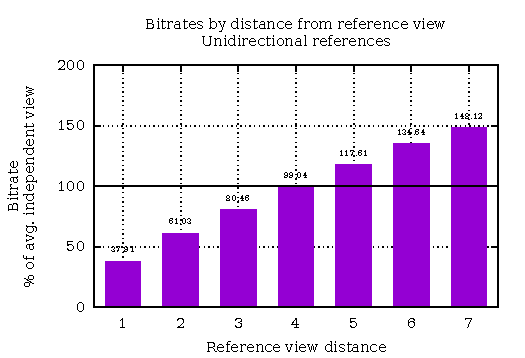
\includegraphics[scale=.68]{figures/motion_vector_data_unconstrained_unidirectional.pdf}
\caption{Average bit-rate for dependent view with one reference by distance
from the reference view.}
\label{fig:uniframes}
\end{figure}

\begin{figure}
\centering
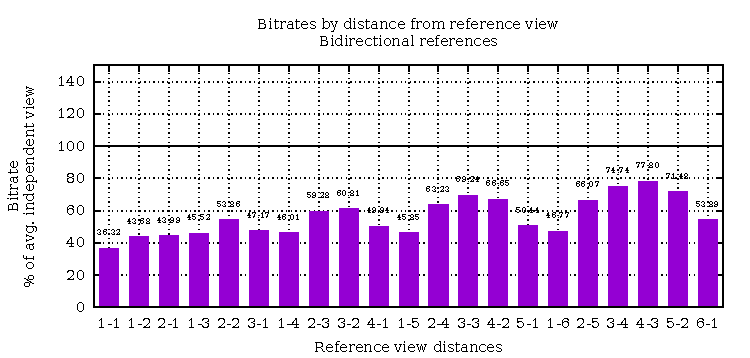
\includegraphics[scale=.68]{figures/motion_vector_data_unconstrained_bidirectional.pdf}
\caption{Average bit-rate for dependent view with two references by distance
from the reference views.}
\label{fig:biframes}
\end{figure}

The first thing to notice is that the bit-rates in these figures are scaled to
percentage of the average independent view. This means that, in figure
\ref{fig:uniframes} for example, once the reference view is four views away,
it is no longer {\it ever} worthwhile to use single-reference motion
compensation in JMVC. It it is at least as cheap to encode the view
independently\footnote{The reader may also notice that the bit-rates are not
quite symmetrical for forward and reverse references. I.e., the bit-rate of
the 5-1 view is slightly larger than the one for the 1-5 view. This is an
artifact of the way JMVC searches List0 and List1 references (the two lists
of references for a B-frame). JMVC slightly prefers List0 motion vectors
regardless of the closeness of the reference frames. So the 1-5 view has
slightly more List0 references than the 5-1 view does List1 references. Since
this is an artifact of the encoder software, we do not take it into account when
deciding on optimal view configurations.}

In figure \ref{fig:biframes}, it's clear that frames with two references scale
more efficiently to the distance of their reference frames. Perhaps
surprisingly, however, a bidirectionally coded view with a distance of one from
either of its references has at most a very slightly better bit-rate than a
unidirectional view with a distance of one from its reference. Since it is
nearly four times as time-consuming, on average, to use two references, this
implies that it is probably never profitable to use a dependent view with an
immediately adjacent references. Instead, bidirectional dependent views should
be used to compensate for being distant from potential references on both sides,
since they scale better to reference distance.

\begin{figure}[H]
\begin{center}
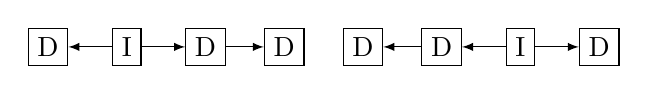
\begin{tikzpicture}[every path/.style={>=latex},every node/.style={draw,rectangle}]
\node            (a) at (0,0)  { D };
\node            (b) at (1,0)  { I };
\node            (c) at (2,0)  { D };
\node            (d) at (3,0)  { D };
\node            (e) at (4,0)  { D };
\node            (f) at (5,0)  { D };
\node            (g) at (6,0)  { I };
\node            (h) at (7,0)  { D };
\draw[->]             (b) edge (a);
\draw[->]             (b) edge (c);
\draw[->]             (c) edge (d);
\draw[->]             (g) edge (h);
\draw[->]             (g) edge (f);
\draw[->]             (f) edge (e);
\end{tikzpicture}
\end{center}
\caption{
Optimal hierarchical configuration of \textbf{I}ndependent and
\textbf{D}ependent views.
}
\label{fig:hierarchical}
\end{figure}

\begin{figure}[H]
\begin{center}
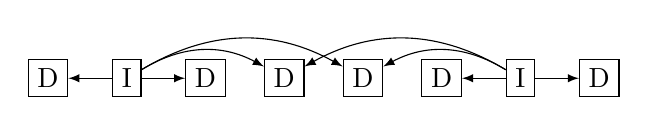
\begin{tikzpicture}[every path/.style={>=latex},every node/.style={draw,rectangle}]
\node            (a) at (0,0)  { D };
\node            (b) at (1,0)  { I };
\node            (c) at (2,0)  { D };
\node            (d) at (3,0)  { D };
\node            (e) at (4,0)  { D };
\node            (f) at (5,0)  { D };
\node            (g) at (6,0)  { I };
\node            (h) at (7,0)  { D };
\draw[->]             (b) edge (a);
\draw[->]             (b) edge (c);
\draw[->, bend left]  (b) edge (d);
\draw[->, bend right] (g) edge (d);
\draw[->]             (g) edge (h);
\draw[->]             (g) edge (f);
\draw[->, bend right] (g) edge (e);
\draw[->, bend left]  (b) edge (e);
\end{tikzpicture}
\end{center}
\caption{
Optimal non-hierarchical configuration of \textbf{I}ndependent and
\textbf{D}ependent views.
}
\label{fig:optimal}
\end{figure}

Based on this information, it seems that the optimal view configuration from the
perspective of bit-rate uses only single reference dependencies, as illustrated
in figure \ref{fig:hierarchical}, which stores eight views in about $4.2$ times
the space of a single independent view. There is one more variable to consider,
however: It may be desirable to be able to split up the views and send just two
of them at a time for stereoscopic video. In this case, the hierarchical
dependencies in figure \ref{fig:hierarchical} would mean that in order to send
views 3 and 4, it would be necessary to send six views in total, using
approximately $3.5$ times the bits of a single independent view.

To deal with this case, we propose the alternative  configuration in figure
\ref{fig:optimal}, which takes up only slightly more space and would require
that at most four views be sent to send any two views. In this case, to send
views 3 and 4 (still the worst case) it would only be necessary to send four
total views, using about $3.2\times$ the bits of a single independent frame.
This is obviously more time-consuming, since B-frames take more than three times
as muchtime to encode as P-frames. We show how this issue can be dealt with
using vertical search constraints in \ref{subsec:constrained}. The
non-hierarchical optimum also takes up slightly more space in total -- about 4.6
times the bits of a single independent frame. It may be worthwhile to make this
trade-off, however, if it makes it less costly to send the views independently.

\begin{figure}[H]
\centering
\begin{subfigure}{.5\textwidth}
\centering
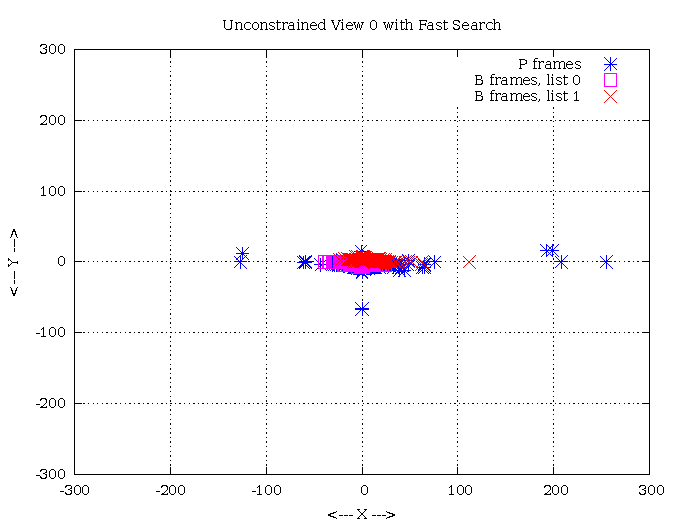
\includegraphics[width=3in]{figures/bedroom1-inter-mvs.pdf}
\caption{Bedroom data set}
\label{fig:bedroom-inter-mvs}
\end{subfigure} \\
\begin{subfigure}{.5\textwidth}
\centering
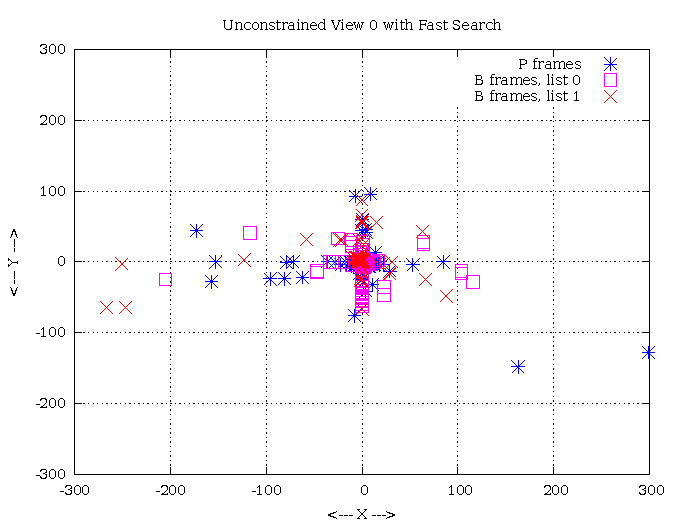
\includegraphics[width=3in]{figures/helicopter-inter-mvs.pdf}
\caption{Helicopter data set}
\label{fig:helicopter-inter-mvs}
\end{subfigure}
\caption{Independent view motion vectors from 2-view test of each data-set.}
\label{fig:inter-mvs}
\end{figure}

\subsection{Distribution of Unconstrained \\ Motion Vectors}
\label{subsec:unconstrained}
In order to determine how well the existing motion-vector search was performing,
we modified JMVC to print out each of the motion vectors it produced for each of
our data sets. We then graphed those motion vectors' positions relative to the
dependent block to show how far afield the encoder was having to look for
satisfactory reference blocks.

Figure \ref{fig:helicopter-inter-mvs} shows the inter motion vectors for the
two-view test helicopter data-set, and \ref{fig:bedroom-inter-mvs} shows the
same for the bedroom data-set. In both cases the motion vectors are clustered
tightly around the location of the dependent block. In the helicopter data set,
motion vectors are both horizontally and vertically displaced with approximately
equal frequency. This is typical of a video with varied motion characteristics.
(The cameras pan right and zoom in as the helicopter flies in from the upper
right and lands.) On the other hand, the motion vectors in the bedroom scene are
mostly located on the x-axis. In this scene, the motion is almost exclusively
horizontal panning. \footnote{The encoder has a bias toward motion vectors
located either directly above or below, or directly to the left or right of the
origin. This is due to the TZ-search algorithm, which searches in a diamond
pattern.}

In both cases, the motion vector search does a good job of taking advantage of
the temporal redundancy between pictures. The inter-frame motion is small enough
that a search centered at the dependent block is able to quickly find appropriate
motion vectors in most cases, with very few motion vectors ending up distant from
the origin.

\begin{figure}[H]
\centering
\begin{subfigure}{.5\textwidth}
\centering
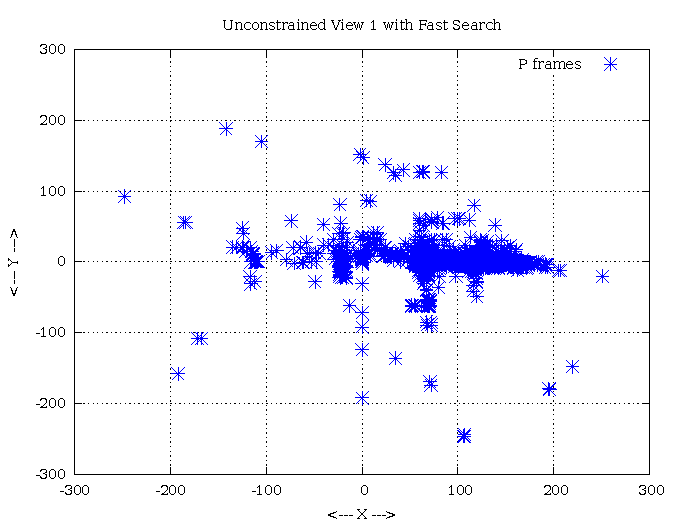
\includegraphics[width=3in]{figures/bedroom1-inter-view-mvs.pdf}
\caption{Bedroom data set}
\label{fig:bedroom-inter-view-mvs}
\end{subfigure} \\
\begin{subfigure}{.5\textwidth}
\centering
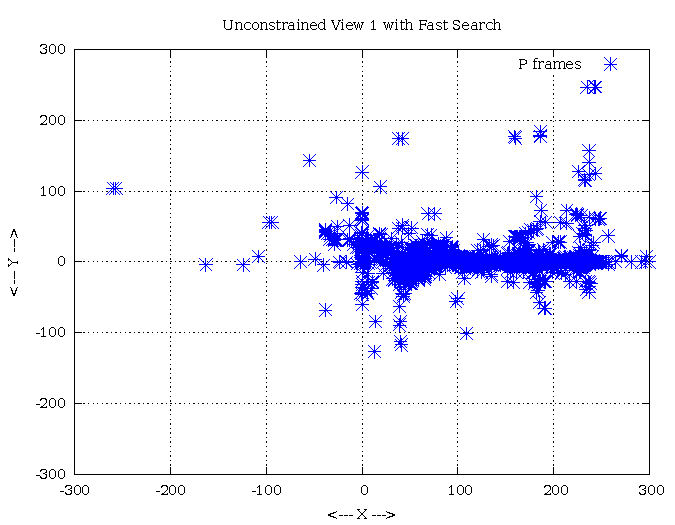
\includegraphics[width=3in]{figures/helicopter-inter-view-mvs.pdf}
\caption{Helicopter data set}
\label{fig:helicopter-inter-view-mvs}
\end{subfigure}
\caption{Dependent view motion vectors from 2-view test of each data-set.}
\label{fig:inter-view-mvs}
\end{figure}

Figure \ref{fig:inter-view-mvs} shows the motion vectors the unmodified JMVC
software produced for the dependent views of the same test. As in the case
of the inter motion compensation in the bedroom data set, the motion vectors
show a tendency to cluster around the x-axis. This reflects the fact that the
reference is horizontally offset from the dependent view. The motion vectors
are much more scattered, however.

Here the diamond refinement used by TZ-search does not do as efficient a job of
finding appropriate motion vectors. This can be attributed to two factors: First,
the ``right'' inter-view reference block according to the view differential is
about 15 pixels away horizontally, a greater distance than is common for
inter motion vectors. This explains why TZ-search comes up with less
well clustered motion vectors in this case that it does for the inter-coded
motion vectors in bedroom data set.

Second, the diamond refinement is spending a lot of time looking at points off
the x-axis. Sometimes, it even finds a reference block that is ``good enough''
in a vertically offset position. Nonetheless, because of the correlation between
views, {\it the best inter-view motion vector is always horizontally displaced,
except in the case of occlusions.} That means that conceptually, the only case in
which searching for inter-view reference blocks off the x-axis is useful is when
an object has been occluded, which accounts for relatively few blocks in most
frames.

\begin{figure}[H]
\centering
\begin{subfigure}{.5\textwidth}
\centering
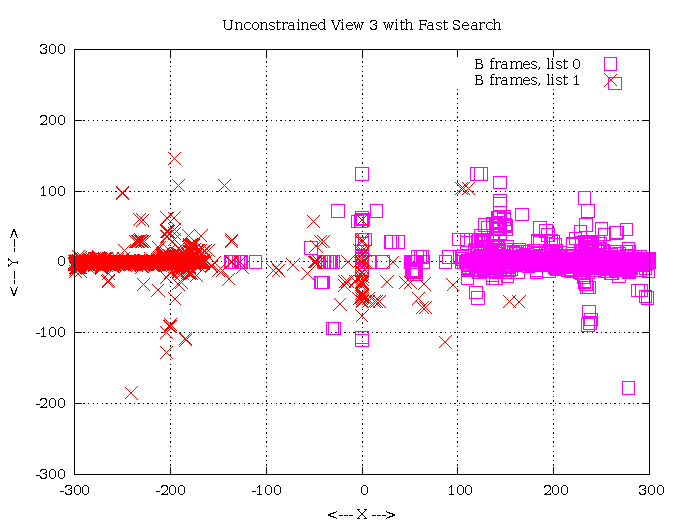
\includegraphics[width=3in]{figures/bedroom1-inter-view-bimvs1.pdf}
\caption{Bedroom data set}
\label{fig:bedroom-inter-view-bimvs1}
\end{subfigure} \\
\begin{subfigure}{.5\textwidth}
\centering
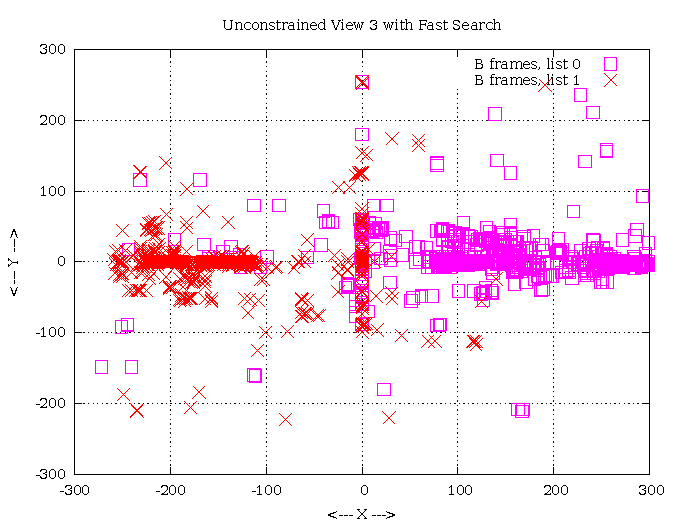
\includegraphics[width=3in]{figures/helicopter-inter-view-bimvs1.pdf}
\caption{Helicopter data set}
\label{fig:helicopter-inter-view-bimvs1}
\end{subfigure}
\caption{Dependent view bidirectional motion vectors from 8-view test of each
data-set.}
\label{fig:inter-view-bimvs1}
\end{figure}

Figure \ref{fig:inter-view-bimvs1} shows similar data for two of the
two-reference views of the non-hierarchical 8-view test. Again, there are a few
motion vectors that lie significantly off the x-axis, but by far the most reflect
the horizontal view offset. Notice that the motion vectors that lie on the x-axis
are centered farther from the origin than they are in \ref{fig:inter-view-mvs}.
This is consistent with the idea that they correspond to view offset, in this
case a greater offset than in \ref{fig:inter-view-mvs}.

\subsection{Benefits of Vertical Constraint}
\label{subsec:constrained}

Inspecting the dependent and reference blocks corresponding to motion vectors
that do not lie on the x-axis, we found that there are two primary reasons these
unexpected motion vectors occur: \begin{compactitem}
\item Some objects, such as the helicopter's shadow as the tree in the helicopter
data set as the camera zooms in, are visible in some views while not being visible
in others. Keeping view-dependencies adjacent minimizes this, but it still occurs.
In this case, allowing motion vectors that aren't on the x-axis can be useful,
since some other block might be a close-enough match.
\item Some blocks are general enough that they have close matches in many blocks
of the reference picture. For example, a section of bedroom wall looks very much
like every other section of bedroom wall. In this case, allowing motion vectors
off of the x-axis is probably not useful; even if the search algorithm happens
to find a vertically offset motion vector, it would likely be able to find one
with no vertical offset as well. \end{compactitem} Under the assumption that the
former case is relatively rare, we propose constraining the motion vector search
to the x-axis.

\begin{figure}[H]
\centering\small
\begin{tabular}{|l|l|l|l|l|}
\multicolumn{1}{c}{} & \multicolumn{2}{c}{unconstrained} & \multicolumn{2}{c}{constrained} \\ \hline
algorithm            & bits            & secs.           & bits            & secs.         \\ \hline
full                 & 20935.92        & 142.58          & 22488.00        & 2.37          \\ \hline
TZ-search            & 21136.80        & 2.72            & 22551.12        & 1.43          \\ \hline
\end{tabular}
\caption{Seconds and bits per encoded frame of the dependent view of the
2-view test using full and TZ-search (100 frames).}
\label{fig:time-full-fast}
\end{figure}

Figure \ref{fig:time-full-fast} shows the time and bits required to encode each
frame using the full and TZ-search algorithms with and without vertical
constraint, and figure \ref{inter-view-constrained-bimvs1} shows the
distribution of the constrained motion vectors using TZ-search. Using the
vertical constraint produces shorter encoding times than using the TZ-search
alone, even when it is accompanied by the brute-force full search algorithm.
Using vertical constraints and TZ-search together produces a speedup of
approximately $47\%$ over using TZ-search alone.

On the other hand, this speedup comes at the cost of a slightly higher bit-rate
-- in the case of the TZ-search, about a $6.7\%$ increase. This increase in
bit-rate is present even when the full search is used, which implies that these
blocks simply have no matching references on the x-axis. That is, it seems that
about $6--7\%$ of the blocks are occluded between these two adjacent views.

\begin{figure}[H]
\centering\small
\begin{subfigure}{.5\textwidth}
\centering
\begin{tabular}{|l|l|l|l|l|l|}
\multicolumn{2}{c}{} & \multicolumn{2}{c}{unconstrained} & \multicolumn{2}{c}{constrained} \\ \hline
view & num. refs.    & bits            & secs.           & bits            & secs.         \\ \hline
0    & 1             & 17503.73        & 2.74            & 17806.24        & 1.45          \\ \hline
2    & 1             & 18294.58        & 2.67            & 18751.60        & 1.44          \\ \hline
3    & 2             & 30397.04        & 11.88           & 30416.96        & 3.03          \\ \hline
4    & 2             & 30430.88        & 11.47           & 30398.82        & 2.93          \\ \hline
5    & 1             & 18661.41        & 2.62            & 19044.34        & 1.51          \\ \hline
7    & 1             & 19802.48        & 2.61            & 20109.01        & 1.48          \\ \hline
\end{tabular}
\caption{Bedroom data set}
\label{fig:bedroom-time-constrained}
\end{subfigure} \\
\begin{subfigure}{.5\textwidth}
\centering
\begin{tabular}{|l|l|l|l|l|l|}
\multicolumn{2}{c}{} & \multicolumn{2}{c}{unconstrained} & \multicolumn{2}{c}{constrained} \\ \hline
view & num. refs.    & bits            & secs.           & bits            & secs.         \\ \hline
0    & 1             & 35027.17        & 2.82            & 35299.28        & 1.34          \\ \hline
2    & 1             & 28179.97        & 2.68            & 28397.52        & 1.33          \\ \hline
3    & 2             & 47177.60        & 11.13           & 47287.41        & 2.64          \\ \hline
4    & 2             & 48463.14        & 11.32           & 48990.05        & 2.66          \\ \hline
5    & 1             & 30080.24        & 2.78            & 30688.85        & 1.34          \\ \hline
7    & 1             & 23016.29        & 2.66            & 23687.09        & 1.33          \\ \hline
\end{tabular}
\caption{Helicopter data set}
\label{fig:helicopter-time-constrained}
\end{subfigure}
\caption{Seconds and bits per encoded frame of the dependent views of the
non-hierarchical 8-view test. Views 1 and 6 (the independent views) are not
included, since we did not constrain the inter motion-vector search.}
\label{fig:time-constrained}
\end{figure}

Figure \ref{fig:time-constrained} contains the times and bit-rates required
to encode each frame of the dependent views of the 8-view hierarchical test.
Views 0, 2, 5, and 7 each have one reference, whereas views 3 and 4 each have
two. For the one-reference views, speedups range from $42.3\%$ (bedroom, view
5) to $52.4\%$ (helicopter, view 0). For the two-reference views, the
constrained version uniformly achieves speedups of about $75\%$. This large
decrease in the time taken to encode bidirectionally coded views serves to
make them more usable in practice: Without vertical constraints, a
two-reference view takes about five times as long as a one reference view, and
probably isn't worth the small decrease in most cases. On the other hand, with
vertical constraints, they now take only about twice as long, so the trade-off
may be worth it.

The penalty in bit-rate varies widely, but in no case is it worse than than a
$2.9\%$ increase, and in most cases it is much less. In fact in one case
(bedroom, view 4), the bit-rate actually decreases in the constrained version.
This implies that whether and by how much the bit-rate will increase is highly
dependent on content.
   
\section{Conclusion} %%%%%%%%%%%%%%%%%%%%%%%%%%%%%%%%%%%%%%%%%%%%%%%%%%%%%%%%%%%
\label{sec:conclusion} %%%%%%%%%%%%%%%%%%%%%%%%%%%%%%%%%%%%%%%%%%%%%%%%%%%%%%%%%
This paper has two main goals: \begin{compactenum}
\item \label{itm:fst} To provide a systematic characterization of view
dependencies, with an eye toward arriving at an optimal dependency structure for
multiview video; and
\item \label{itm:snd} To examine the usefulness of applying vertical constraints
to inter-view motion-vector search. \end{compactenum}

With respect to \ref{itm:fst}, we have provided timing data for each view type,
averaged over several trials and two data sets, and bit-rate data for each
dependent view type, categorized by their distances from their reference views.
Base on this data, we presented two optimal view dependency structures: a
hierarchical one with minimal bit-rate overall, and a non-hierarchical one to
make it cheaper to transmit a subset of the views. Lastly, we demonstrated that
bidirectionally coded views can scale more effectively to view distance, but
come at a hefty cost in time. Fortunately, vertically constraining inter-view
motion vectors can drastically reduce the time they take, making them more
practical.

With respect to \ref{itm:snd}, using vertical constraints can provide
significant speedups with a small increase in bit-rate, due to occlusions. 
In particular, they provide about a four-times speedup for bidirectionally
coded views. The speedup they provide is large enough that this could be a
reasonable trade-off, especially for time-sensitive applications, like streaming
video.

\bibliographystyle{abbrv}
\bibliography{bibliography}

\end{document} %%%%%%%%%%%%%%%%%%%%%%%%%%%%%%%%%%%%%%%%%%%%%%%%%%%%%%%%%%%%%%%%%
%%%%%%%%%%%%%%%%%%%%%%%%%%%%%%%%%%%%%%%%%%%%%%%%%%%%%%%%%%%%%%%%%%%%%%%%%%%%%%%%
